%%Things to do
%%Papers to read:
%%Caviarres papers
%%Geum paper Ecology Letters
%%Xia Xiao's paper from geum
%%Schob (Spain) cost and benefit of facilitation
%%Brad's SEM paper and the Nature paper


%%0) Write-up and get larger dataset from Brad
%%1) What does this mean ecologically? Also, how does this analysis
%%parallel more common analyses of diversity?
%%2) Prep a presentation for Richard
%%3) Prep presentation for the group


\documentclass[12pt]{article}
\usepackage{geometry}                % See geometry.pdf to learn the layout options. There are lots.
\geometry{letterpaper}                   % ... or a4paper or a5paper or ... 
%\geometry{landscape}                % Activate for for rotated page geometry
%\usepackage[parfill]{parskip}    % Activate to begin paragraphs with an empty line rather than an indent
\usepackage{graphicx}
\usepackage{amssymb}
\usepackage{/Library/Frameworks/R.framework/Resources/share/texmf/Sweave}


\title{Intraspecific variation influences community network structure: Tracing the roots of interactions to genetics.}
\author{M.K. Lau, R. Michalet and the Alpine Pals Group}
%\date{}                                           % Activate to display a given date or no date

\begin{document}
\maketitle


%\setcounter{tocdepth}{3}
%\tableofcontent

%Chateaubriand Fellowship INFO
%User ID: 1669994985

\section{Summary}

%\subsection{Understanding the structure of individual interaction networks is important}
%\begin{itemize}
%\item Indirect effects (examples, Mistletoe-Juniper-Solitaire, Jamie's paper)
%\item Weak interactions and linking communities
%\item Links between structure and stability of communities
%\item Advances in network modeling techniques (Reverse Engineering)
%\item Theoretical Frameworks (Small Worlds, Weak Interactions,, Modularity)
%\item A rich amount of data on behavioral ecologies exists for many taxa that can be synthesized into qualitative models of species interactions
%\item Cohen's paper on beyond tri-trophic interactions
%\item Food-web research (Bascompte, Dunne, Martinez, Schmidt, May, Pimm, Paine, Darwin)
%\item Joe's paper on tri-trophic interactions
%\item Phylogenetics and species interactions (Rezende et al. 2007 Nature)
%\end{itemize}


\subsection{Study Proposal}

\begin{itemize}
\item Using existing data of abundances of facilitated species inside
  and outside of the nurse genotypes, generate an estimate of the
  dependency of each species to each genotype

\item Compare the network facilitation network structure given
  different abundances of open and closed genotypes:

\item Primary Questions:
  \begin{enumerate}
  \item Is there an overall preponderance of nestedness or modularity?
  \item Are their bio-geographic patterns of network structure?
  \item Are their phylogenetic patterns of network structure (for both
    the nurse plants and the beneficiary species)?
  \end{enumerate}
\end{itemize}


\section{Individual level facitilation network models}

%%Run the models the first time you run the document through Sweave
 
%\subsection{Dependencies}

%%%Add these functions to the CorNets package


%%Source your functions

\section{Import Data}

%%%Data were provided by the Apling Pals Group with permission from
%%%Ray Callaway and others. Robbin Brooker provided the access to the
%%%data. Brad Butterfield provided .csv files that he had
%%%updated. Brad Cook helped to facilitate data acquisition.

\begin{Schunk}
\begin{Sinput}
> mywd <- getwd()
> setwd("data")
> cush.data <- list()
> for (i in 1:length(dir())) {
+     cush.data[[i]] <- read.csv(dir()[i])
+ }
> names(cush.data) <- paste(lapply(cush.data, function(x) colnames(x)[2]), 
+     dir(), sep = "_")
> setwd(mywd)
> as.character(unique(unlist(lapply(cush.data, function(x) x[, 
+     4]))))
> for (i in 1:length(cush.data)) {
+     cush.data[[i]][is.na(cush.data[[i]])] <- 0
+ }
> cush.data <- lapply(cush.data, function(x) data.frame(x[, 1:4], 
+     rm.spp(x[, 5:ncol(x)], n = 10)))
\end{Sinput}
\end{Schunk}

\section{Build Models}

\begin{Schunk}
\begin{Sinput}
> if (run.rii == TRUE) {
+     cush.rii <- list()
+     cush.rii <- lapply(cush.data, function(x) rii(x[, 5:ncol(x)], 
+         rep = x[, 3], site = x[, 4], decreasing = FALSE))
+     any(is.na(unlist(cush.rii)))
+     any(as.logical(lapply(cush.rii, function(x) all(x == 0))))
+     names(cush.data)[as.logical(lapply(cush.rii, function(x) all(x == 
+         0)))]
+ } else {
+ }
\end{Sinput}
\begin{Soutput}
NULL
\end{Soutput}
\end{Schunk}


\section{Ratios of Positive and Negative RII}


% latex table generated in R 2.12.1 by xtable 1.5-6 package
% Thu Nov 10 15:11:32 2011
\begin{table}[ht]
\begin{center}
\begin{tabular}{rrrrr}
  \hline
 & Estimate & Std. Error & t value & Pr($>$$|$t$|$) \\ 
  \hline
(Intercept) & 18.0620 & 2.9575 & 6.11 & 0.0000 \\ 
  unlist(neg.rii) & 0.7130 & 0.1213 & 5.88 & 0.0000 \\ 
   \hline
\end{tabular}
\end{center}
\end{table}
\section{Network Structure Metrics}


\subsection{Nestedness}

\begin{Schunk}
\begin{Sinput}
> cush.zeros <- as.logical(lapply(cush.rii, function(x) all(x == 
+     0)))
> length(cush.rii[cush.zeros != TRUE])/length(cush.rii)
\end{Sinput}
\begin{Soutput}
[1] 0.9090909
\end{Soutput}
\begin{Sinput}
> if (run.rii == TRUE) {
+     cush.nest <- lapply(cush.rii, function(x) nested(web = abs(x), 
+         method = "NODF"))
+ } else {
+ }
\end{Sinput}
\begin{Soutput}
NULL
\end{Soutput}
\begin{Sinput}
> cush.nest <- as.numeric(cush.nest)
> length(cush.nest)
\end{Sinput}
\begin{Soutput}
[1] 77
\end{Soutput}
\begin{Sinput}
> total.rii <- as.numeric(I(as.numeric(pos.rii) + as.numeric(neg.rii)))
\end{Sinput}
\end{Schunk}


% latex table generated in R 2.12.1 by xtable 1.5-6 package
% Thu Nov 10 15:11:32 2011
\begin{table}[ht]
\begin{center}
\begin{tabular}{rrrrr}
  \hline
 & Estimate & Std. Error & t value & Pr($>$$|$t$|$) \\ 
  \hline
(Intercept) & -0.0129 & 0.1143 & -0.11 & 0.9102 \\ 
  as.numeric(pos.rii) & 0.0296 & 0.0030 & 9.80 & 0.0000 \\ 
   \hline
\end{tabular}
\end{center}
\end{table}
% latex table generated in R 2.12.1 by xtable 1.5-6 package
% Thu Nov 10 15:11:32 2011
\begin{table}[ht]
\begin{center}
\begin{tabular}{rrrrr}
  \hline
 & Estimate & Std. Error & t value & Pr($>$$|$t$|$) \\ 
  \hline
(Intercept) & 0.4844 & 0.1221 & 3.97 & 0.0002 \\ 
  as.numeric(neg.rii) & 0.0253 & 0.0050 & 5.05 & 0.0000 \\ 
   \hline
\end{tabular}
\end{center}
\end{table}
% latex table generated in R 2.12.1 by xtable 1.5-6 package
% Thu Nov 10 15:11:32 2011
\begin{table}[ht]
\begin{center}
\begin{tabular}{rrrrr}
  \hline
 & Estimate & Std. Error & t value & Pr($>$$|$t$|$) \\ 
  \hline
(Intercept) & 0.1055 & 0.1126 & 0.94 & 0.3518 \\ 
  total.rii & 0.0181 & 0.0020 & 9.09 & 0.0000 \\ 
   \hline
\end{tabular}
\end{center}
\end{table}

\section{Modularity}
%%Look for modules in the unipartite represntations
\subsection{Unipartite: Individuals}

\begin{Schunk}
\begin{Sinput}
> library(sna)
\end{Sinput}
\begin{Soutput}
     Tools for Social Network Analysis
Version      2.2-0 created on      2010-11-21.
copyright (c) 2005, Carter T. Butts, University of California-Irvine
Type help(package="sna") to get started.
\end{Soutput}
\begin{Sinput}
> cush.iug <- lapply(cush.rii, as.one.mode, project = "lower")
> cush.mod <- list()
> cush.mod
\end{Sinput}
\begin{Soutput}
list()
\end{Soutput}
\begin{Sinput}
> pos.iug <- cush.rii
> for (i in 1:length(pos.iug)) {
+     pos.iug[[i]][pos.iug[[i]] < 0] <- 0
+ }
> pos.iug <- lapply(pos.iug, as.one.mode, project = "lower")
\end{Sinput}
\end{Schunk}

\begin{figure} 
\begin{center} 
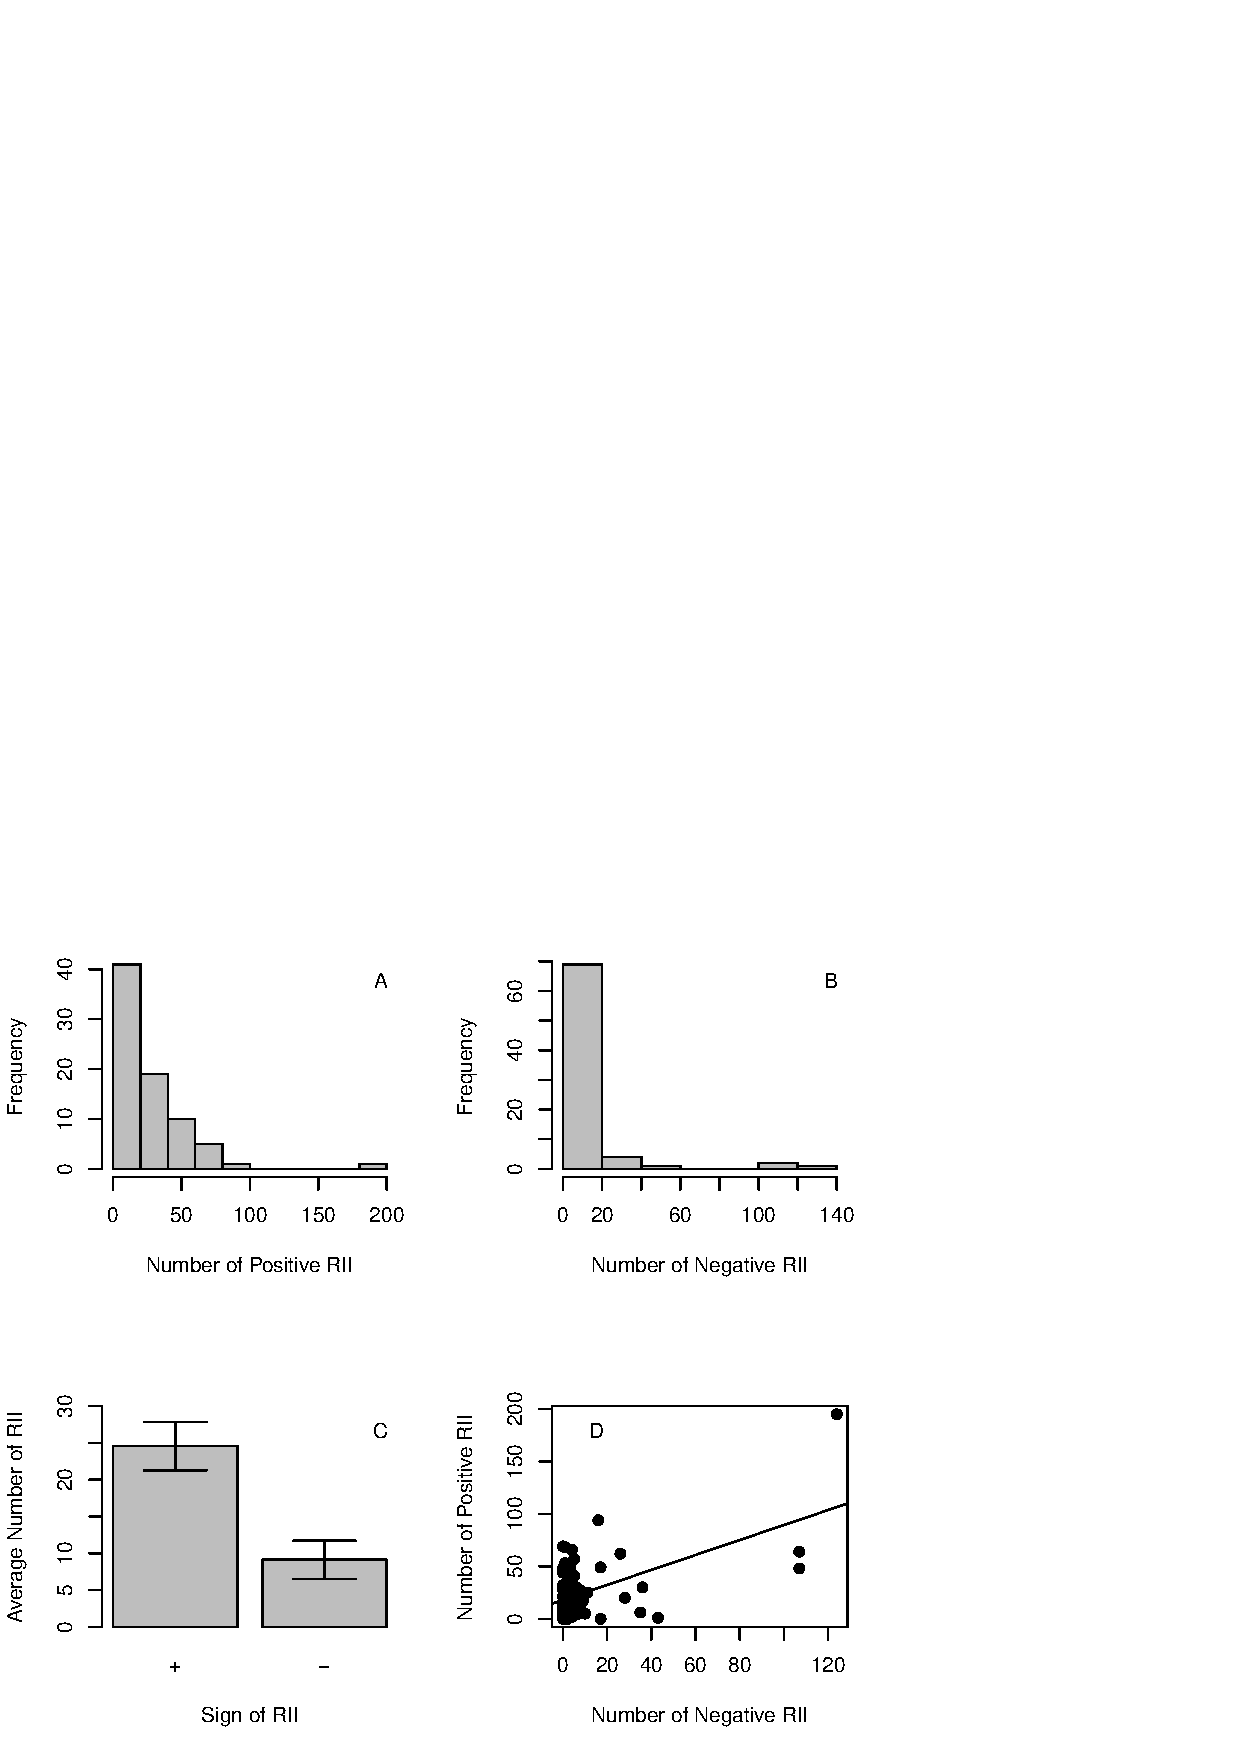
\includegraphics{GoFN-fig1}
\end{center} 
\caption{}
\label{fig:one}
\end{figure}

\begin{figure} 
\begin{center} 
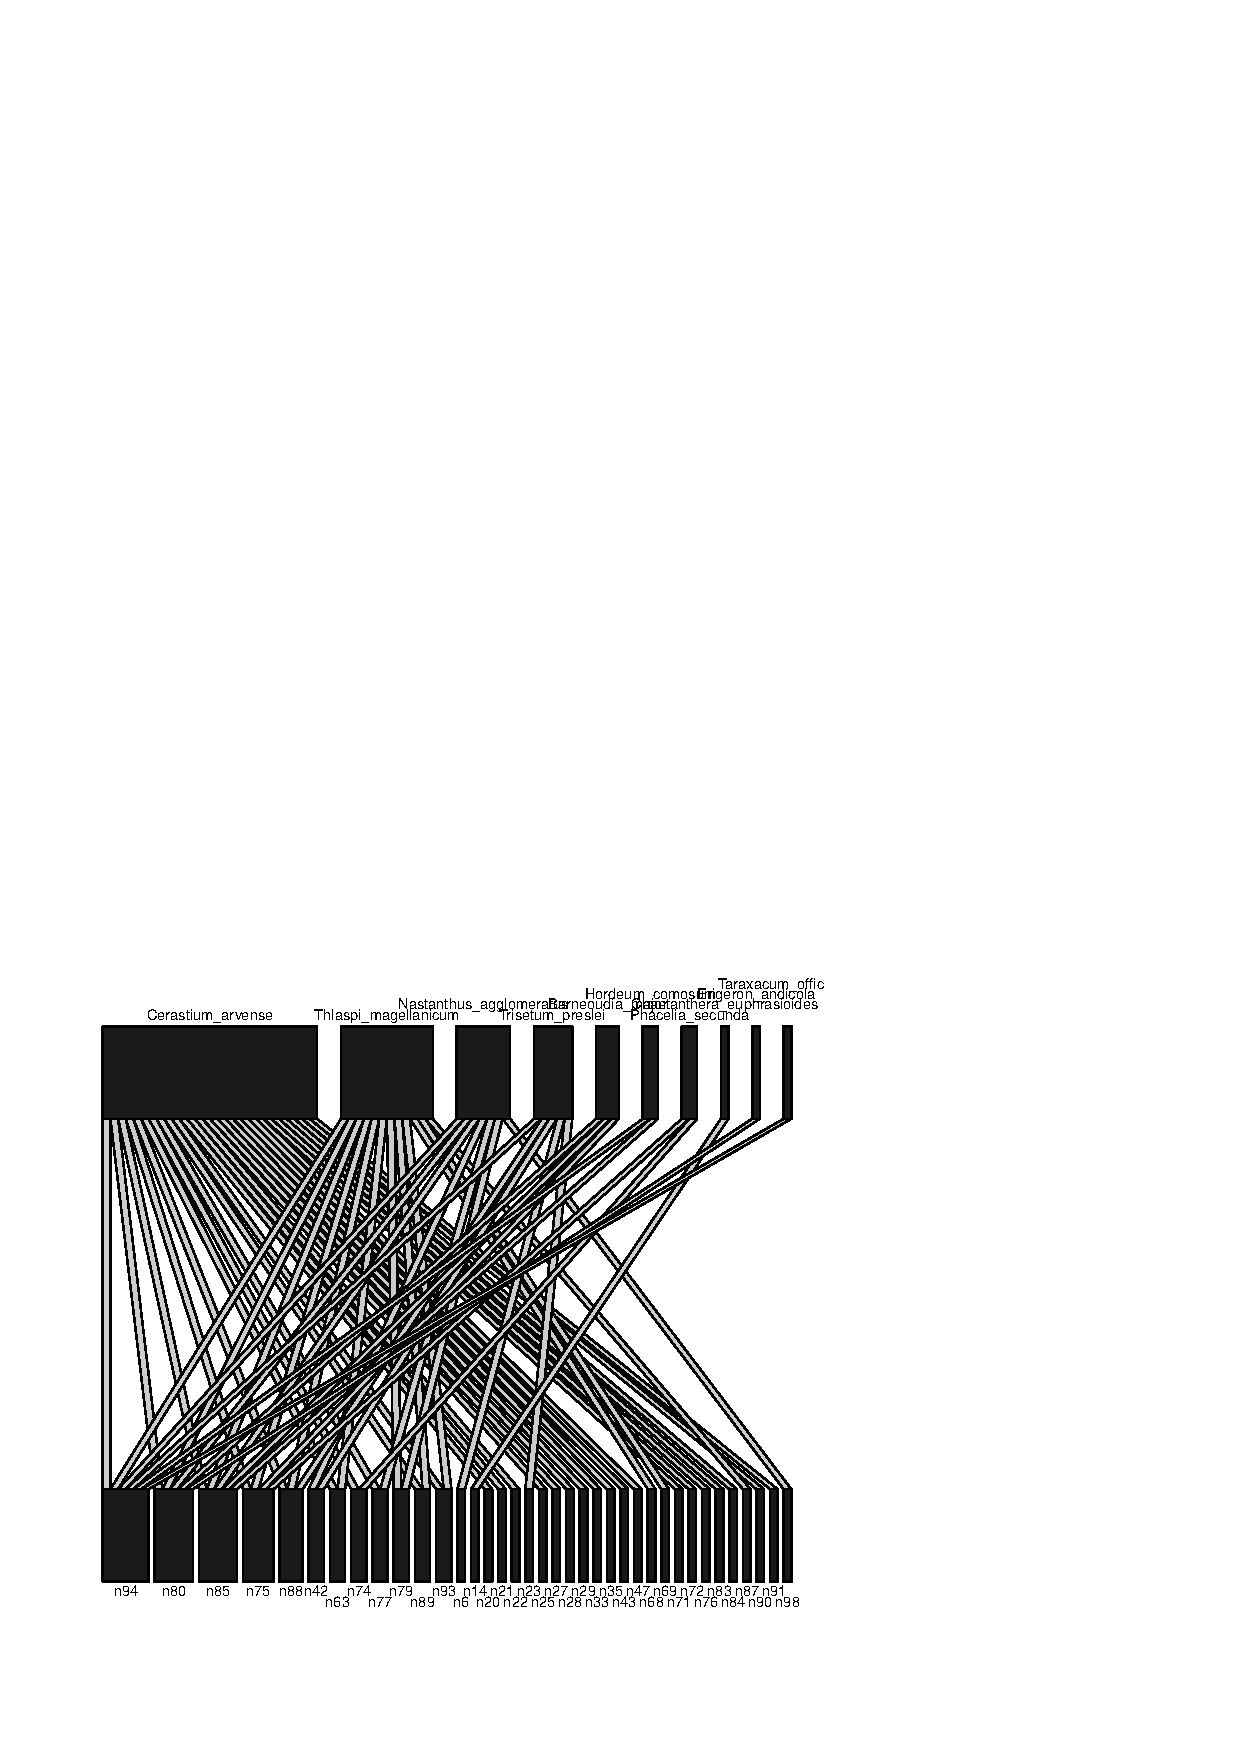
\includegraphics{GoFN-fig2}
\end{center} 
\caption{}
\label{fig:two}
\end{figure}

\begin{figure} 
\begin{center} 
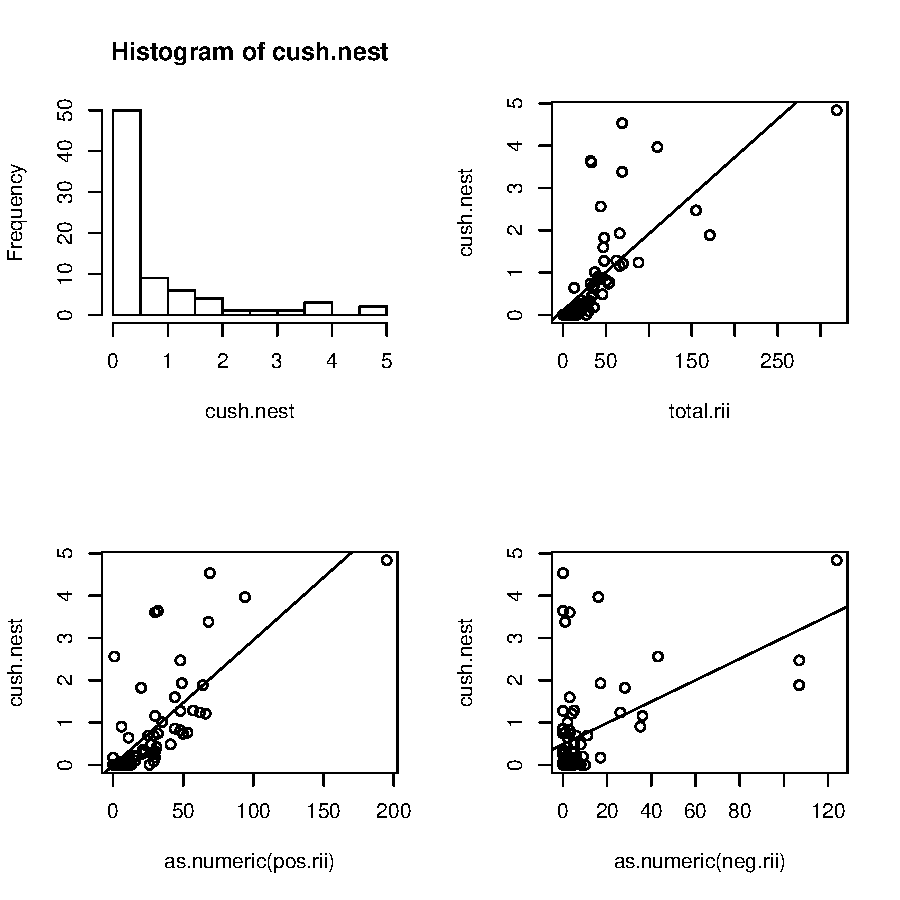
\includegraphics{GoFN-fig3}
\end{center} 
\caption{}
\label{fig:three}
\end{figure}




\end{document}


%% ##No need to use database access programs. The easiest means was to work around by exporting all data tables from the database as .csv files.
%% ##NOTE: instead of accessing the database directly, it worked best to export the data tables to csv files. This was a nightmare of convoluted dead ends. It may be that you need to purchase some software or drivers to get the RODBC or Hmisc functions to work. The Hmisc looked the most promising, but it repeatedly produced errors saying that there were invalid characters.
%% ##library(RODBC) 
%% ##library(Hmisc)
